%%%%%%%%%%%%%%%%%%%%%%%%%%%%%%%%%%%%%%%%%%%%%%%%%%%%%%%%%%%%%%%%%%%%%%%%%%%%%%%%


%\documentclass[letterpaper, 10pt, conference]{IEEEtran}
\documentclass[letterpaper, 10pt, conference]{ieeeconf}
\IEEEoverridecommandlockouts
\overrideIEEEmargins 
\usepackage[table]{xcolor}
\usepackage{tikz}
\usetikzlibrary{calc,decorations.markings,arrows, fadings}
\usepackage{tikz-timing}
\usepackage[top=1in,bottom=1in,right=1in,left=1in]{geometry}
\usepackage{amsmath}
\usepackage{xifthen}
\usepackage{amsfonts}
\usepackage{tabu}
\usepackage{graphicx,dblfloatfix}
\usepackage[font=small]{caption}
\usepackage{subcaption}
\usepackage{cite}
\usepackage{placeins}
\usepackage{xspace}
\usepackage{subfiles}
\usepackage{url}
\usepackage[outline]{contour}
\contourlength{0.18em}

% Packages for including pseudo-code
\usepackage{algorithmicx}
\usepackage{algorithm}
\usepackage{algpseudocode}

% Nice Little macro for adding a comment box. Include incrementing comment numbers.
\newcounter{comcount}
\setcounter{comcount}{0}
\newcommand{\mycomment}[1]
{
\refstepcounter{comcount}
\smallskip\noindent\fbox{\parbox{\linewidth}{\emph{Comment \arabic{comcount}} : \small{#1}}} 
}

\newcommand{\spx}{\mathcal{S}}

%
%Once I break this in to multiple sections, each section will be added with:
%	\subfile{filename}
%In those other files, I have as preamble:
%	\documentclass[main.tex]{subfiles}
%

\title{\LARGE \bf
A Stick-Slip Omnidirectional Powertrain for Low-Cost Swarm Robotics: Mechanism, Calibration, and Control
}

\author{John Klingner, Anshul Kanakia, Nicholas Farrow, Dustin Reishus and Nikolaus Correll%
\thanks{Department of Computer Science,
University of Colorado at Boulder,
 Boulder, CO 80309,
{\tt\small firstname.lastname{@}colorado.edu}}%
}

\newcommand{\Tau}{\boldsymbol{\mathrm{T}}}

\begin{document}
\maketitle


%%%%%%%%%%%%%%%%%%%%%%%%%%%%%%%%%%%%%%%%%%%%%%%%%%%%%%%%%%%%%%%%%%%%%%%%%%%%%%%%
\begin{abstract}
We present an omnidirectional powertrain for swarm robotic platforms that relies on low-cost vibration motors. We describe a mechanism and controller to achieve full 3-DoF motion on the plane. The proposed approach does not require the motors to be in phase, and overcomes differences in manufacturing by a hardware-in-the-loop auto-calibration routine based on the Nelder-Mead algorithm, which issues motion commands via infrared and records the resulting trajectories using an off-the-shelf webcam. We show convergence results of the calibration routine and sample trajectories of the swarm robotic platform ``Droplet'' demonstrating turning and omnidirectional drive.   
\end{abstract}

%\keywords{Swarm robotics, low-cost, hopping robot, bristle-bot principle}

%%%%%%%%%%%%%%%%%%%%%%%%%%%%%%%%%%%%%%%%%%%%%%%%%%%%%%%%%%%%%%%%%%%%%%%%%%%%%%%%
\section{Introduction}
We present a low-cost miniature robot powertrain that approximates omnidirectional motion using three vibration motors. Classically, miniature robotic platforms such as r-one \cite{mclurkin2013low}, Jasmine \cite{jasmine} and Alice \cite{alice} require geared motors, which are expensive and difficult to miniaturize. The proposed powertrain is a variant of the ``stick-slip'' actuator that has been introduced in \cite{breguet1998stick}, and has been shown to be particularly attractive for high precision movements \cite{brufau2005micron,chu2006novel,martel2001three,martel2005fundamental,eigoli2012locomotion} and force control \cite{vartholomeos2008analysis}.   

Whereas stick-slip actuators traditionally require changing their length, e.g., using piezo ceramics,  \cite{breguet1998stick, martel2005fundamental}, a similar effect can be achieved using a vibration motor, an effect well-known from the ``Bristle-bot'' series of toys. The simplicity and availability of this actuator  has led to its use on low-cost miniature robot platforms, such as the Kilobots, \cite{rubenstein2012kilobot} based on the design presented in \cite{Vartholomeos2006}, which approximates the dynamics of a differential wheel platform (see also \cite{spartali2013speed} for additional analysis). Achieving fully holonomic motion on the plane requires at least three vibration motors, however. Whereas \cite{Vartholomeos2005} proposes a symmetric three-motor design and its analysis, their approach requires all motors to be in phase, which is not feasible on a low-cost platform. This paper addresses these problems by presenting a design, controller and calibration routine that allows omnidirectional motion on a ping-pong ball sized robot ``Droplet'' (Figure \ref{Droplets}).

\begin{figure}[!htb]
	\centering
		\includegraphics[width=0.8\columnwidth]{./Images/Droplets.png}
	\caption{The Droplet swarm robotics platform. Two Droplets are shown, one with the cover removed. A penny is included for scale. The background is the floor of alternating power and ground strips from which the Droplets draw power.}
	\label{Droplets}
\end{figure}
%%%%%%%%%%%%%%%%%%%%%%%%%%%%%%%%%%%%%%%%%%%%%%%%%%%%%%%%%%%%%%%%%%%%%%%%%%%%%%%%
\section{The Droplet Swarm Robotic Platform}
The Droplets are an open-source swarm robotic platform, with source code and manufacturing information available online\footnote{\url{https://github.com/correlllab/cu-Droplet}}. Each Droplet is a spherical, roughly ping-pong ball sized robot with a radius of $2.2\,\mathrm{cm}$ and a flat bottom. They have three extended headers for legs located symmetrically around the robot. The legs are spaced $120^\circ$ apart, $15.1\, \mathrm{mm}$ from the center. Mounted symmetrically opposite the legs are coin-type vibration motors (\emph{Hochar}) arranged as shown in Figure~\ref{fig:PWMs}. The  motors  are circular, $10\,\mathrm{mm}$ in diameter and $2.7\,\mathrm{mm}$ thick, weigh $1.1\,\mathrm{g}$, rated at $3\,\mathrm{V}$ DC, vibrate at $200\pm42\,\mathrm{Hz}$, and of the type commonly used in cell phones and pagers. As locomotion is not their primary intent, the vibration motors used here have low manufacturing consistency for rotation speed and direction. In bulk, they cost around $\$0.50$ each.
\begin{figure*}[hb]
\setcounter{figure}{2}
\centering
\subfile{singleDoFModel}
\caption{Simple 1DoF model of motion principle. Horizontal motion of the mass causes the platform to scoot right and left. The vertical motion of the mass effects the magnitude of the friction experienced by the platform as it scoots. Thus, the platform experiences net motion over a full rotation, in a direction determined by the rotation's direction \cite{Vartholomeos2005}.}
\label{motorDiagram}
\end{figure*}
\begin{figure}[h]
\setcounter{figure}{1}
	\centering
	\subfile{motorLocations}
	\caption{An image of the Droplet's shell and vibration motors in place. The locations where the legs are mounted are labeled.}
	\label{fig:PWMs}
\setcounter{figure}{3}
\end{figure}

The Droplets use an Atmel Xmega128A3U microcontroller. Motors are controlled via a Allegro A3901 dual H-Bridge that is driven by a pulse-width modulated (PWM) signal generated by the microcontroller. This setup allows us to provide a series of precise pulses as well as changing the direction of rotation. A 6-directional infrared communication and range and bearing system \cite{farrow14} is also present on the Droplets. They receive power via their legs through a floor with alternating strips of $+5V$ and $GND$.
%%%%%%%%%%%%%%%%%%%%%%%%%%%%%%%%%%%%%%%%%%%%%%%%%%%%%%%%%%%%%%%%%%%%%%%%%%%%%%%%
\section{Principle of Operation}

\subsection{1-DoF Stick-slip Motion}
A vibration motor is a DC motor with a mass on the shaft, such that the center of mass is not on the axis of rotation. Spinning the motor throws the mass around, causing motion of the entire motor body due to inertia. As the mass swings through its circular path, the motor experiences a force towards that mass. Over a full rotation, the net force experienced by the motor is 0.

If we neglect friction, the platform will slide backwards and forwards due to the backwards and forwards forces from the mass, but experiences no net translation. With friction, the vertical forces of the mass become relevant. The downward force of gravity is mitigated by the upward force from the swinging mass. Crucially, this means that the total downward force experienced by the platform is lower while the mass is swinging upwards, and the effects of friction are reduced. The direction of the horizontal force during this period of reduced friction (or, the direction the motor is spinning) determines the direction of travel. See also \cite{Vartholomeos2005,Vartholomeos2006} for a mathematical treatment of this model. Figure~\ref{motorDiagram} illustrates this process. Note that the robot does not actually need to jump up, as long as the upward force sufficiently reduces static friction. 

\subsection{Motion Principle Applied to Droplets}
Combining the 1-DoF actuator described above with others to obtain a 3-DoF robotic platform is not trivial as it requires all motors to be in phase \cite{Vartholomeos2005}, and is infeasible with low-cost hardware. In \cite{Vartholomeos2005}, the motors are positioned next to the legs. Our design positions the motors on the opposite side of the platform's center of mass from the legs (Figure~\ref{DropletMotorDiagram}). With this configuration, the forces from an individual motor cause the platform to pivot about the leg opposite of this motor. Our proposed locomotion scheme combines a sequence of individual pivots, with only one motor on at a time. This allows us to overcome the limitations of the motors being in phase described in \cite{Vartholomeos2005}.

\begin{figure}[h]
\centering
\subfile{DropletDiagram}
\caption{Arrangement of vibration motors $m_1, m_2$ and $m_3$ and legs $l_1, l_2$ and $l_3$.}
\label{DropletMotorDiagram}
\vspace{-0.5em}
\end{figure}

\subsection{Forward and inverse kinematics}
In order to model this platform using traditional kinematics, we assume that individual pivot motions happen not sequentially but simultaneously. Whereas each pivot motion happens at the maximal speed of the motor, we can approximate the effective rotational speeds $\dot{\theta}_i$ around leg $i$ by introducing delays of varying length after each microscopic pivot. Assuming that low-level control of $\dot{\theta}_i$ and switching between pivot motions happens much faster than actual motion, we can reduce the proposed mechanism to a circular robot with three standard wheels, albeit without kinematic constraints, at the same location and orientation as the motors shown in Figure~\ref{DropletMotorDiagram}, and with retractable legs. Here, the absence of kinematic constraints lets the standard wheels skid frictionlessly in any direction, while the retractable legs allows enabling and disabling pivot points, modeling the up and down movements of the platform. 

In this reduced model, each motor $m_1$, $m_2$, and $m_3$ controls the angular velocity $\dot{\theta}_1$, $\dot{\theta}_2$ and $\dot{\theta}_3$ around its associated pivot point opposite of the motor. This lets us derive the following forward kinematic equations in the robot coordinate frame $\dot{x}_r$, $\dot{y}_r$ and $\dot{\theta}_r$.
We assume the $x$-axis to be orthogonal to the spinning direction of motor 1, and the $y$-axis orthogonal to the $x$-axis, as seen in Figure~\ref{DropletMotorDiagram}. Following the right-hand rule, the $z$-axis is pointing downwards, and the direction of $\theta$ is clockwise around the robot's origin. As the speed at the mounting point of motor $m_i$ is given by $\ell \theta_i$, with $\ell$ the distance from the motor to the robot's center, and its direction tangential to the Droplet, we can calculate each motor's contribution to the speed at the robot's center as follows:
\begin{align}\label{eq:fwd}
\dot{x}_r &=  \ell \dot{\theta}_2 \cos(210^o) + \ell \dot{\theta}_3 \cos(-30^o)\notag\\
\dot{y}_r &=  \ell \dot{\theta}_1  +\ell \dot{\theta}_2 \sin(210^o) +\ell \dot{\theta}_3 \sin(-30^o)\\
\dot{\theta}_r &= \dot{\theta}_1 + \dot{\theta}_2 + \dot{\theta}_3\notag  
\end{align}
Here, we assume positive $\theta_i$ to be aligned with the direction of thrust of motor $m_i$. That is, if all motors spin in the same direction, they all contribute to $\dot{\theta}_r$ in the same way. Notice that motor 1 does not contribute to $\dot{x}_r$ as it spins orthogonally to the x-axis.

Equation \ref{eq:fwd} is a linear system with three unknowns, and we can solve for $\dot{\theta}_1$, $\dot{\theta}_2$ and $\dot{\theta}_3$:
\begin{align}\label{eq:ik}
\dot{\theta}_1 &=  \frac{2}{3}\frac{\dot{y}_r}{\ell} + \frac{\dot{\theta}_r}{3}\notag\\
\dot{\theta}_2 &= -\frac{\sqrt{3}}{3}\frac{\dot{x}_r}{\ell} - \frac{1}{3}\frac{\dot{y}_r}{\ell} + \frac{\dot{\theta}_r}{3}\\
\dot{\theta}_2 &= \frac{\sqrt{3}}{3}\frac{\dot{x}_r}{\ell} - \frac{1}{3}\frac{\dot{y}_r}{\ell} + \frac{\dot{\theta}_r}{3}\notag
\end{align}

The rotational velocity values from \eqref{eq:ik} can now be transformed to motor values supplied to the Droplet to achieve desired motion in the $\{\dot{x}_r, \dot{y}_r, \dot{\theta}_r\}$ coordinate frame using auto-calibration techniques discussed in the following section. The reader is referred to \cite{balkcom2006time} for a thorough analysis of time-optimal trajectories of omni-drive vehicles. 

%%%%%%%%%%%%%%%%%%%%%%%%%%%%%%%%%%%%%%%%%%%%%%%%%%%%%%%%%%%%%%%%%%%%%%%%%%%%%%%%
\section{Auto-Calibration}
A challenge arising from low-cost hardware is that achieving equal step sizes requires tedious calibration.
It would be possible to calibrate each platform manually, but this platform is motivated by a desire for low-cost, large scale robot swarms.  Manual calibration of a swarm of thousands of robots would be completely impractical, and so we automate the process. 

\subsection{Experimental Setup}
The motors are kept at a fixed $100\%$ duty cycle. Each step, we turn a motor on for a fixed amount of time, $t_{\text{on}}$, plus some offset, $\tau$,  which varies for each motor direction. Next, all motors are off for a fixed amount of time, $t_{\text{off}}$. Figure~\ref{fig:pwmSignals} shows this in more detail. We denote the vector of calibration values for each motor direction $\Tau=\{\tau_1, \tau_2, \tau_3\}$. Calibration is done by changing the $\tau$ values such that the pivot induced by the motors is the same. These values are integers of magnitude $^1/_{32}\,\mathrm{ms}$. For our platform, $t_{\text{on}}$ is $30\,\mathrm{ms}$, which was determined to be the minimum amount of time required to induce pivoting for a typical motor. Similarly, $t_{\text{off}}$ is the time required for vibrations of the system to settle---a shorter off time causes platform instability. For our platform, $t_{\text{off}}$ is $10\,\mathrm{ms}$.

\begin{figure}[!htb]
\centering
\subfile{PWMfigure}
\caption{The PWM signals for motion in the negative $y$ direction for motors $m_1$ \& $m_2$. $m_3$ is inactive during this motion. If both A and B are high, the motor is braking. If both are low, the motor is inactive. If only one signal is high, the motor rotates in that direction.}
\label{fig:pwmSignals}
\end{figure}

\begin{figure}[!htb]
\centering
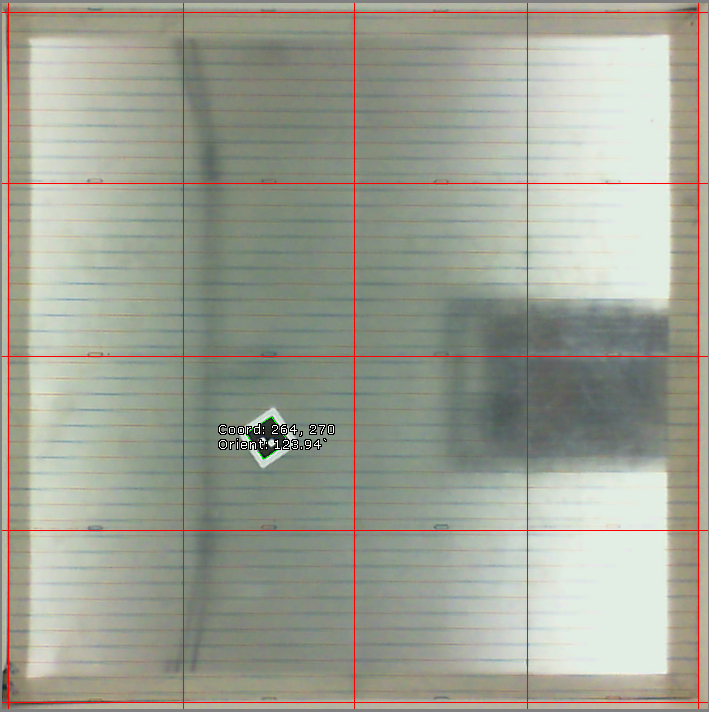
\includegraphics[width=0.8\linewidth]{images/cameraView}
\caption{View from the overhead camera onto the Droplet equipped with a fiducial marker that can be recognized by RoboRealm.\label{fig:expsetup}} 
\end{figure}

Data is collected using a high resolution USB camera\footnote{Microsoft LifeCam Cinema}, and motion-tracking software RoboRealm~\cite{RoboRealm}. A fiducial marking is secured to the top of the platform to aid in tracking and orientation calculations (Figure~\ref{fig:expsetup}). Specifically, we collect the global position and orientation of the Droplet in each frame.

To update the Droplet's calibration settings, we find the least-squares best-fit circle of the collected coordinates. Specifically, the circle's radius and whether that circle's center is to the Droplet's left or right. While calibrating for walking straight, we optimize for maximizing the radius of the fitted circle (if the Droplet traveled perfectly straight, the radius would by infinite). When calibrating for spinning, we optimize for minimizing the radius of the fitted circle (a perfect spin would have radius 0).

We communicate with and control the platform through a serial-to-IR transmitter. 

\subsection{Calibration Method}
\begin{algorithm}
\caption{Automated method for calibrating an individual Droplet's rotational motion}
\begin{algorithmic}
	\Function{Auto\_Calibrate}{$dir, \alpha, \beta$}		
		\State $\spx \gets$ init\_simplex\_guess()
		\State $[\tau^*_1,\tau^*_2, \tau^*_3] \gets$ Nelder\_Mead($\spx, dir, \alpha, \beta$) 
		\State write\_to\_memory($id_{robot}, dir, \tau^*_1,\tau^*_2, \tau^*_3$)
	\EndFunction
	\Function{Nelder\_Mead}{$\spx, dir, \alpha, \beta$}
		\State $radii \gets$ new list()
		\State $v \gets$ new list()
		\For{$\vec{\tau}$ in $\spx$}
			\State $radii$.push(get\_robot\_spin\_circle\_est($\vec{\tau}, dir$))
			\State $v$.push(get\_robot\_spin\_vel\_est($\vec{\tau}$))
		\EndFor
		\State $\spx' \gets$ new\_simplex\_est($\spx, radii, v, dir, \alpha, \beta$)
		\If{within\_tolerence($\spx', radii, v$)}
			\State \Return best\_values($\spx'$)
		\Else
			\State Nelder\_Mead($\spx', \alpha, \beta$)
		\EndIf
	\EndFunction
\end{algorithmic}\label{alg:spx}
\end{algorithm}

We use the Nelder-Mead Simplex algorithm \cite{NelderMead} to calibrate motor parameters for spinning in a given direction (clockwise or anti-clockwise), as seen in Alg.(\ref{alg:spx}). 

The simplex algorithm looks for a set of motor parameters $\Tau=\{\tau_1, \tau_2, \tau_3\}$ that minimize the following equation:
\begin{equation}
\alpha R_{\mathrm{circ}}(\Tau) - \beta V_{\mathrm{rot}}(\Tau)\label{eq:maxcal}
\end{equation}
where $R_{\mathrm{circ}}(\Tau)$ is the radius of the circle fitted to the robot's motion with parameters $\Tau$ and $V_{\mathrm{rot}}(\Tau)$ is the angular velocity of the robot's motion with those parameters. $\alpha$ and $\beta$ are weighting constants such that $\alpha > \beta$, as we prefer motor values that minimize circle radius over rotational speed.

The Nelder-Mead algorithm attempts to provide iteratively better motor control parameters by solving the optimization problem \eqref{eq:maxcal} until a sufficiently accurate set of parameters is provided that falls within the desired tolerances of rotational circle radius and velocity, or it converges to a local minimum. It then returns the optimal $\Tau$, denoted $\Tau^{*}=\{\tau^{*}_1,\tau^{*}_2,\tau^{*}_3\}$.

Additionally, this method identifies which motors are ``flipped''---i.e., which motors spin opposite from what is expected, because having the motor directions flipped results in a large radius. Once we have clockwise spin calibrated, this is equivalent to having three matched pivot sizes for the motors' clockwise spins. To finish calibrating, we just need to find counterclockwise values that match the clockwise ones. This is done for each motor independently by having the Droplet walk straight in a direction. Now, we want to maximize the radius of  the circle traced by the Droplet. As the Droplet improves straight-line motion accuracy, the radius of the circle transcribed by its motion approaches $\infty$. A binary search is performed over the space of possible clockwise values for each motor.

Note that since the Nelder-Mead algorithm also treats flipped motors, it's possible for it to find a minima with all motors flipped, spinning in the counterclockwise direction. The rest of the algorithm is performed symmetrically in this case.

%%%%%%%%%%%%%%%%%%%%%%%%%%%%%%%%%%%%%%%%%%%%%%%%%%%%%%%%%%%%%%%%%%%%%%%%%%%%%%%%
\begin{figure}[htb!]
\centering
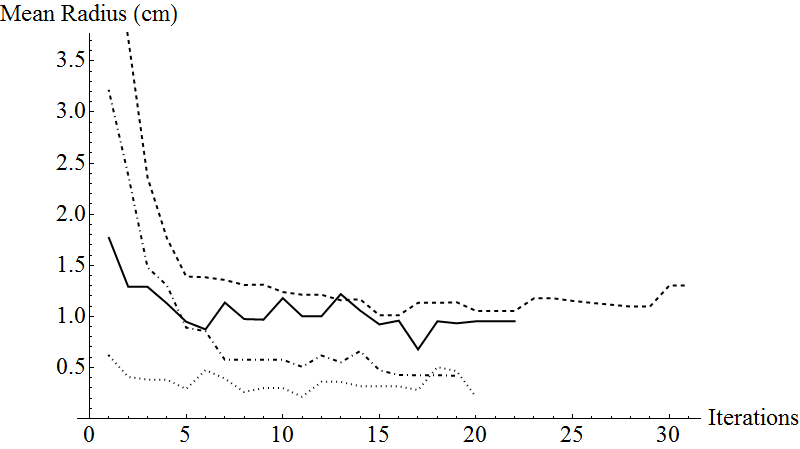
\includegraphics[width=\linewidth]{Images/radiiConverging.png}
\caption{The mean of the best three points of the simplex after each pass through the Nelder-Mead optimization loop, shown for four different Droplets. After the optimization converges or a particularly good value is found, the motors are set to the best of all settings tested.}
\label{fig:radiiConverging}
\end{figure}

\section{Results}
\subsection{Calibration}
We performed calibration for four different Droplets. Figure \ref{fig:radiiConverging} shows convergence of the optimization routine, and Table~\ref{DropletValueTable} shows a sample of calibrated values. This demonstrates the variability of the individual robots.

\begin{table}[htb!]
\centering
\begin{tabular}{r|c|c|c|c|c|c}
 ID & $\tau_1$ & $-\tau_1$ & $\tau_2$ & $-\tau_2$ & $\tau_3$ & $-\tau_3$ \\
\hline
15 & 68 & -1 & 56 & -5 & \cellcolor{gray!15} 40 & \cellcolor{gray!15} 0\\ 
18 & 84 & -89 & 84 & 202 & \cellcolor{gray!15} 128 & \cellcolor{gray!15} 290\\
11 & -96 & 83 & 64 & 62 & -289 & 55
\end{tabular}
\caption{Sample of calibrated values for specific Droplets. Shaded cells indicate that that particular motor was flipped. $-\tau_i$ is used to indicate the reverse value for that motor.}
\label{DropletValueTable}
\vspace{-1em}
\end{table}

\subsection{Motion}
For a more robust demonstration of the calibrated Droplet's performance, we performed two additional experiments. Figure~\ref{fig:squareWalk} shows two attempts of a Droplet walking in a square pattern, produced by walking forward and turning $90^\circ$ to the right repeatedly. For the solid trial, with desired square size of $8\,\mathrm{cm}$, this resulted in a final position error of $2.75\,\mathrm{cm}$ and a final orientation error of $27^\circ$. For the dashed trial, with desired square size $6.5\,\mathrm{cm}$, this resulted in a final position error of $1.4\,\mathrm{cm}$ and final orientation error of $39^\circ$.

Figure~\ref{fig:triangleWalk} shows two attempts of a Droplet walking a triangle pattern. This is done without rotations, using the two degrees of translational freedom. Both trials have a nominal side length of $6\,\mathrm{cm}$. The final position errors were $3.28\,\mathrm{cm}$ and $2.77\,\mathrm{cm}$ for the solid and dashed paths respectively.

\begin{figure}[htb!]
\centering
\includegraphics[width=0.9\linewidth]{Images/DropletWalksSquare}
\caption{Two attempts (solid, dashed) of a calibrated Droplet walking in a square, combing straight motion with a rotation.}
\label{fig:squareWalk}
\end{figure}
\begin{figure}[htb!]
\centering
\includegraphics[width=0.9\linewidth]{Images/DropletWalksTriangle}
\caption{Two attempts (solid, dashed) of a calibrated Droplet walking in a triangle without rotation. The two attempts are aligned such that the Droplets start with the same position and orientation.}
\label{fig:triangleWalk}
\end{figure}

%%%%%%%%%%%%%%%%%%%%%%%%%%%%%%%%%%%%%%%%%%%%%%%%%%%%%%%%%%%%%%%%%%%%%%%%%%%%%%%%
\section{Discussion}
The proposed control scheme relies on running the vibration motors at full speed for a brief moment of time. What this timing should be is an outcome of the optimization routine. While this approach leads to acceptable results and a wide range of possible motions, it is not necessarily optimal with respect to speed and power consumption. For example, we could also vary the voltage provided to the motors using a high-frequency PWM signal, which might lead to even better speed/power performance. We wish to explore this and other control schemes in future work, though increasing the search space is generally undesirable for a hardware-in-the-loop optimization scheme.  

It should be emphasized that the results in Figures~\ref{fig:squareWalk} and \ref{fig:triangleWalk} are open-loop; one drawback to stick-slip motion is that we have no odometry to reduce error propagation. This can be addressed, however, by exploiting ranging information from nearby static robots as is demonstrated by \cite{rubenstein2012kilobot} for a similar platform.

Calibrating the Droplets via an overhead camera and off-the-shelf computer vision software allows us to obtain results quickly and potentially scales to calibration of multiple robots at the same time. An alternative approach would be to rely on the Droplets' range-and-bearing system \cite{farrow14} which would potentially allow a large number of Droplets to calibrate in parallel without additional hardware. 

The proposed forward and inverse kinematics are an approximation as the robots do not move in straight lines, but using a sequence of pivoting steps. While this effect is negligible over distances in the order of the robot's diameter, it is prohibitive to reach the accuracies that the stick-slip drive is capable of. For example, when ``spinning in place'', the robots' coordinate system moves in a radius in the order of millimeters. In the future, we wish to explore motion planning techniques to improve accuracy by combining a sequence of pivoting motions, much like a knight on a chess board needs to do to reach a neighboring cell. 

\section{Conclusion}
We presented an omni-directional powertrain and miniature robotic platform that relies on low-cost vibration motors. We have shown how we can overcome challenges with synchronization and manufacturing variability, which have thus far prevented this approach from practical viability. 

Whereas the proposed auto-calibration allows us to make up for manufacturing variability, it still requires significant manual labor to calibrate individual platforms, which is tedious for swarms with thousands of robots that we envision. In the future, we will therefore investigate methods to calibrate robots collaboratively and online.  

\section*{Acknowledgments} We thank Dr.\ Timothy Caldwell and Prof.\ Matthew Mason for helpful discussion on suitable optimization methods and kinematics, respectively.   
This work has been supported by NSF award \#1150223 and a CI fellowship to D. Reishus.


\bibliographystyle{ieeetr}
\bibliography{mybibfile}

\end{document}

